\chapter{Differenzierbarkeit}
\Mark{Chapter 4.1}
$f$: $D \ra \R$ stetig dann bedeutet dies, dass $f$ in $D$ keine \ggq{Spr�nge} hat\\
$f$: $D \ra \R$ differenzierbar bedeutet, dass $f$ in $D$ keine Spr�nge und keine \ggq{Knicke} hat

\begin{fdefinition}[Differenzierbarkeit]
Die Funktion $f$: $D \ra \R$ hei�t im Punkt $x_0 \in D$ \indexb{differenzierbar}, falls der Grenzwert
\[f' (x_0) \ceq \lim_{x \ra x_0} \frac{f(x) - f(x_0)}{x - x_0}\]
existiert $(f' (x_0) \in \R)$.\\
Die Zahl $f'(x_0)$ hei�t dann \indexb{Ableitung} von $f$ an der Stelle $x_0$.\\
Die Funktion $f$: $D \ra \R$ hei�t differenzierbar in $A \subseteq D$, falls $f$ in jedem $x_0 \in A$ differenzierbar ist.
\Mark{Definition 4.1}
\end{fdefinition}
\section*{Geometrische Interpretation}
\begin{center}
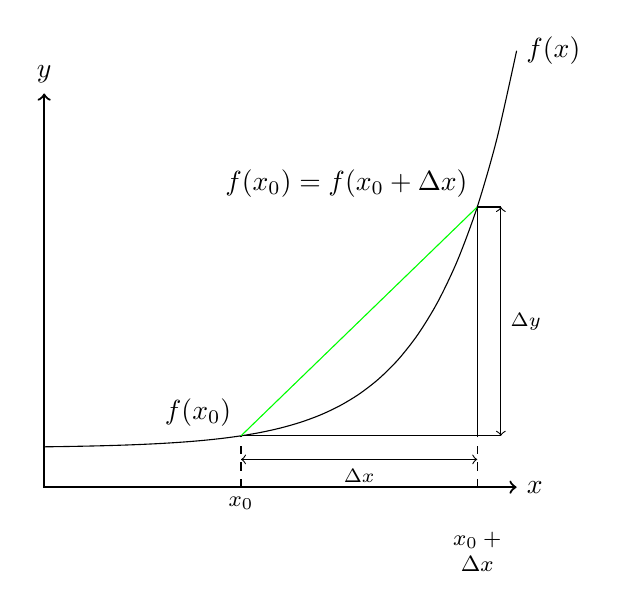
\begin{tikzpicture}[domain=0:6]
\draw[<->,thick] (0,5) node[above] {$y$} -- (0,0) -- (6,0) node[right] {$x$};
\draw plot[smooth] (\x,{exp(\x)/80 + 0.5}) node[right] {$f(x)$};
\draw (2.5,{exp(2.5)/80 + 0.5}) -- (5.5,{exp(2.5)/80 + 0.5}) -- (5.5,{exp(5.5)/80 + 0.5});
\draw[color=green] (2.5,{exp(2.5)/80 + 0.5}) node[above left, color=black] {$f(x_0)$} -- (5.5,{exp(5.5)/80 + 0.5}) node[above left, color=black] {$f(x_0) = f(x_0 + \Delta x)$};
\draw[dashed] (2.5,0) node[below] {\footnotesize{$x_0$}} -- (2.5,{exp(2.5)/80 + 0.5});
\draw[dashed] (5.5,0) node[below, text width=7mm] {\begin{center}\footnotesize{$x_0 + \Delta x$}\end{center}} -- (5.5,{exp(5.5)/80 + 0.5});

\draw[<->] (2.5,{exp(2.5)/80 + 0.2}) -- (5.5,{exp(2.5)/80 + 0.2}) node[below, midway] {\scriptsize{$\Delta x$}};
\draw (5.5,{exp(2.5)/80 + 0.5}) -- (5.8,{exp(2.5)/80 + 0.5});
\draw (5.5,{exp(5.5)/80 + 0.5}) -- (5.8,{exp(5.5)/80 + 0.5});
\draw[<->] (5.8,{exp(2.5)/80 + 0.5}) -- (5.8,{exp(5.5)/80 + 0.5}) node[right, midway] {\scriptsize{$\Delta y$}};
\end{tikzpicture}
\end{center}
\Img{MA2-28.04.2009-IMG-1}

Mit $h = \Delta x$ stellt der Differenzenquotient
\[\frac{f(x_0 + \Delta x) - f(x_0)}{\delta x} = \frac{f(x_0 + h) - f(x_0)}{h} = \frac{\Delta y}{\Delta x} = \frac{\Delta f}{\Delta x}\]
die Steigung der Sekante (Sehne) zwischen $f(x_0)$ und $f(x_0 + \Delta x)$ dar.\\
F�r $h \ra 0$ \ac{bzw.} $\Delta x \ra 0$ geht die Sekante in die Tangente in $x_0$ �ber und Steigung der Tangente ist
\begin{align*}
f'(x_0) &= \frac{df(x)}{dx}_{x = x_0} = \frac{df}{dx}_{(x_0)} = \lim_{\Delta x \ra 0} \frac{f(x + \Delta x) - f(x_0)}{\Delta x}\\
&=\tanx{\alpha}
\end{align*}

\begin{bemerkung}
\mbox{}\par
\begin{enumerate}
\item In Anlehnung an d en Differenzenquotient $\frac{\Delta f}{\Delta x}$ nennt man $\frac{df}{dx}$ \indexb{Differenzialquotient}.
\item $h$ \ac{bzw.} $\Delta x$ muss nicht $> 0$ sein.
\item Alternative Definition der Differenzierbarkeit\\
		Sei $D \subseteq \R$ und $x_0 \in D$, so dass mindestens eine Folge $(x_n)_{n \in \N}$ mit $x_n \in D \backslash \gklamm{x_0}$ existiert mit $\lim_{n \ra \un} (x_n) = x_0$.\\
		Eine Funktion $f$: $D \ra \R$ hei�t differenzierbar in $x_0 \in D$, falls es eine Konstante $a \in \R$ und eine Funktion $r$: $D \ra \R$ mit $\lim_{x \ra x_0} r(x) = 0$ gibt, sodass
		\[f(x) = f(x_0) + a \mal (x - x_0) + r(x) \mal (x - x_0)~~x \in D\]
		In diesem Fall ist $a = f' (x_0)$

\item Die Gleichung der Tangente an $f$ in $x_0$ lautet
		\[\ub{T(f, x)}{= T(x) = T_f(x)} = f(x_0) + f' (x_0) \mal (x - x_0)\]

\item aus 3, 4 folgt, dass sich lokal (also in der N�he eines gegebenen Punktes $x_0$) der \ggq{Zuwachs} der Funktion $f$ durch den Zuwachs der Tangente $T_f$ ($a_n$ $f in x_0$) darstellen l�sst.
		\begin{align*}
		\Delta f &= f(x) - f(x_0)\\
		&= f(x_0) + f'(x_0) (x - x_0) + r(x) \mal (x - x_0) - f(x_0)\\
		&= f'(x_0) \mal (x - x_0) + r(x) \mal (x - x_0)\\
		&\approx f'(x_0) \mal (x - x_0)\\
		&= T_f(x) - T_f(x_0)\\
		\Ra& df = f'(x) dx \tx{ Differential}
		\end{align*}
		\ac{d.h.} wenn man um die Infinitesimale Gr��e $dx$ von $x_0$ weggeht, �ndert sich der Funktionswert um $df = f'(x_0) dx$
\end{enumerate}
\end{bemerkung}

\begin{beispiel}
\mbox{}\par
\begin{enumerate}
\item $f(x) = 4x - 5$\\
		Ist $f$ in $x_0 = 3$ differenzierbar?\\
		Ist $f$ in $\R$ differenzierbar?
		\begin{align*}
		\lim_{x \ra x_0} \frac{f(x) - f(x_0)}{x - x_0} &= \lim_{h \ra 0} \frac{f(x_0 + h) - f(x_0)}{h}\\
		&= \lim_{h \ra 0} \frac{\rkl{4 (x_0 + h) - 5} - (4 x_0 - 5)}{h}\\
		&= \lim_{h \ra 0} \frac{4x_0 + 4h - 5 - 4x_0 + 5}{h} = \lim_{h \ra 0} 4 = 4
		\end{align*}
		Da der Grenzwert existiert ohne dass wir den Wert von $x_0$ gebraucht h�tten, ist $f$ in ganz $\R$ differenzierbar.
\end{enumerate}
\end{beispiel}

\section{Aufgabe 4.1}
\label{sec:Differenzierbarkeit_A4_1}
Ermitteln sie die Ableitung der Funktion $f(x) = x^2$ direkt mit Hilfe der Definition

L�sung siehe \vref{sec:Differenzierbarkeit_A4_1L}.
\Solved{Link zu L�sung}

\begin{beispiel}
\mbox{}\par
\begin{enumerate}[start=2]
\item $f(x) = e^x$ gesucht $f'(x)$
		\begin{align*}
		\lim_{x \ra x_0} \frac{f(x) - f(x_0)}{x - x_0} &= \lim_{h \ra 0} \frac{f (x_0 + h) - f(x_0)}{h}\\
		&= \lim_{h \ra 0} \frac{e^{x_0 + h} - e^{x_0}}{h} = \lim_{h \ra 0} \frac{e^{x_0} e^h - e^{x_0}}{h}\\
		&= e^{x_0} \mal \lim_{h \ra 0} \frac{e^h - 1}{h} = e^{x_0} \lim_{h \ra 0} \frac{1}{h} \rkl{\sum_{k = 0}^{\un} \frac{h^k}{k!} - 1}\\
		&= e^{x_0} \mal \lim_{h \ra 0} \rkl{\frac{1}{h} \sum_{k = 1}^{\un} \frac{h^k}{k!}} = e^{x_0} \ub{\lim_{h \ra 0} \sum_{k = 1}^{\un} \frac{h^{k - 1}}{k!}}{= \tx{\textcircled{$\star$}}}\\
		\tx{\textcircled{$\star$}} &\klgl \lim_{h \ra 0} \sum_{k = 1}^{\un} \frac{\betrag{h}^{k - 1}}{k!} = \lim_{h \ra 0} \sum_{k = 0}^{\un} \frac{\betrag{h}^k}{(k + 1)!} \klgl \lim_{h \ra 0} \sum_{k = 0}^{\un} \frac{\betrag{h}^k}{k!}\\
		&= \lim_{h \ra 0} e^{\betrag{h}} = 1\\
		\tx{\textcircled{$\star$}} &= \lim_{h \ra 0} \frac{h^k}{(k + 1)!} = \lim_{h \ra 0} \rkl{1 - \sum_{k = 1}^{\un} \frac{\betrag{h}^k}{(k + 1)!}}\\
		&= \lim_{h \ra 0} \rkl{1 - \sum_{k = 1}^{\infty} \frac{\betrag{h}}{2} \mal \frac{\betrag{h}}{3} \mal \frac{\betrag{h}}{4} \dots \frac{\betrag{h}}{(k + 1)}} \grgl \lim_{h \ra \infty} \rkl{1 - \sum_{k = 1}^{\infty} \rkl{\frac{\betrag{h}}{2}}^k}\\
		&= \lim_{h \ra 0} \rkl{1 - \frac{\betrag{h}}{2} \mal \sum_{k = 0}^{\un} \rkl{\frac{\betrag{h}}{2}}^k}\\
		&= \lim_{h \ra 0} \rkl{1 - \frac{\betrag{h}}{2} \mal \frac{1}{1 - \frac{\betrag{h}}{2}}}\\
		&= 1 - \lim_{h \ra 0} \frac{\betrag{h}}{2} \mal \lim_{h \ra 0} \frac{1}{1} - \frac{\betrag{h}}{2} = 1 - 0 \mal 1 = 1\\
		\Ra& \frac{d}{dx} \rkl{e^x}_{x = x_0} = e^{x_0} = f'(x_0)\\
		\Ra& f'(x) = e^x
		\end{align*}
\end{enumerate}
\end{beispiel}

\begin{fsatz}[Stetigkeit differenzierbarer Funktionen]
Die Funktion $f$: $D \ra \R$ sei im Punkt $x_0 \in D$ differenzierbar. Dann ist $f$ in $x_0$ auch stetig.
\Mark{Satz 4.2}
\end{fsatz}

\begin{fbeweis}
\begin{align*}
\lim_{x \ra x_0} f(x) &= \lim_{x \ra x_0} \rkl{f (x_0) + f'(x_0) \mal (x - x_0) + r(x) \mal (x - x_0)}\\
&= f(x_0) + f'(x_0) \mal \ub{\lim_{x \ra x_0} (x - x_0)}{= 0} + \ub{\lim_{x \ra x_0} (r(x))}{=0} \mal \ub{\lim_{x \ra x_0} (x - x_0)}{=0}\\
&= f(x_0)
\end{align*}\qed
\end{fbeweis}

\begin{fsatz}[Rechenregeln f�r Ableitungen]
Die Funktionen $f$ und $g$ seien im Punkt $x_0$ differenzierbar und $\alpha, \beta \in \R$. Dann gilt:
\begin{enumerate}[label=\roman*)]
\item Die Funktion $\alpha \mal f + \beta \mal g$ ist in $x_0$ differenzierbar und f�r die Ableitung gilt:
		\[\rkl{a \mal f + \beta \mal g}' (x_0) \rkl{=\frac{d}{dx} \rkl{\alpha \mal f (x) + \beta \mal g(x)}_{x = x_0}} = \alpha f'(x_0) + \beta \mal g'(x_0)\]

\item Die Funktion $f \mal g$ ist in $x_0$ differenzierbar und f�r die Ableitung gilt:
		\[(f \mal g)' (x_0) = f'(x_0) \mal g(x_0) + f(x_0) \mal g'(x_0)\]
		\indexb{Produktregel}

\item Falls $g(x_0) \neq 0$, ist die Funktion $\frac{f}{g}$ an der Stelle $x_0$ differenzierbar und f�r die Ableitung gilt die \indexb{Quotientenregel}
		\[\rkl{\rac{f}{g}}' (x_0) = \frac{f'(x_0) \mal g(x_0) - f(x_0) \mal g'(x_0)}{\rkl{g(x_0)}^2}\]
\end{enumerate}
\end{fsatz}

\begin{fbeweis}
\mbox{}\par
\begin{enumerate}[label=\roman*)]
\item -
\item \begin{align*}
		\frac{(f \mal g)(x) - (f \mal g) (x_0)}{x - x_0} &= \frac{f(x) \mal g(x) - f(x_0) \mal g(x_0)}{x - x_0}\\
		&= \frac{f(x) \mal g(x) - f(x_0) \mal g(x) + f(x_0) \mal g(x) - f(x_0) \mal g(x_0)}{x - x_0}\\
		&= \ubl[18mm]{g(x)}{$\ural{x \ra x_0} g(x)$\\\textcolor{blue}{da $g$ in $x_0$ stetig (da $g$ in $x_0$ \ac{differenz.})}} \mal \ubl{\frac{f(x) - f(x_0)}{x - x_0}}{$\ural{x \ra x_0} f'(x_0)$\\\textcolor{blue}{da $f$ in $x_0$ \ac{differenz.}}} + f(x_0) \mal \ubl{\frac{g(x) - g(x_0)}{x - x_0}}{$\ural{x \ra x_0} g'(x_0)$\\\textcolor{blue}{da $g$ in $x_0$ \ac{differenz.}}}\\&\ural{x \ra x_0} f'(x_0) \mal g(x_0) + f(x_0) \mal g'(x_0)
		\end{align*}

\item Spezialfall $f = 1$ (\Lra $f(x) = 1 \forall x$)
		\begin{align*}
		\frac{\frac{1}{g} (x) - \frac{1}{g} (x_0)}{x - x_0} &= \frac{\frac{1}{g(x)} - \frac{1}{g(x)}}{x - x_0}\\
		&= \ubl[18mm]{g(x)}{$\ural{x \ra x_0} g(x)$\\\textcolor{blue}{da $g$ in $x_0$ stetig (da $g$ in $x_0$ \ac{differenz.})}} \mal \ubl{\frac{f(x) - f(x_0)}{x - x_0}}{$\ural{x \ra x_0} f'(x_0)$\\\textcolor{blue}{da $f$ in $x_0$ \ac{differenz.}}} + f(x_0) \mal \ubl{\frac{g(x) - g(x_0)}{x - x_0}}{$\ural{x \ra x_0} g'(x_0)$\\\textcolor{blue}{da $g$ in $x_0$ \ac{differenz.}}}\\&\ural{x \ra x_0} f'(x_0) \mal g(x_0) + f(x_0) \mal g'(x_0)
		\end{align*}
		Allgemeiner Fall $\frac{f}{g} = f \mal \frac{1}{g}$\\
		Verwendung der Produktregel
		\begin{align*}
		\rkl{\frac{f}{g}}' (x_0) = \rkl{f \mal \frac{1}{g}}' x_0 &= f' (x_0) \mal \frac{1}{g(x_0)} + f(x_0) \mal \rkl{\frac{1}{g}}' (x_0)\\
		&= \frac{f'(x_0)}{g(x_0)} + f(x_0) \mal \rkl{- \frac{g'(x_0)}{\rkl{g(x_0)}^2}}\\
		&= \frac{f' (x_0) \mal g(x_0) - f(x_0) \mal g'(x_0)}{\rkl{g(x_0)}^2}
		\end{align*}
\end{enumerate}
\end{fbeweis}

\begin{beispiel}
\mbox{}\par
\begin{enumerate}
\item Behauptung: $\forall n \in \N$: $\rkl{x^n}' = n \mal x^{n - 1}$
		Beweis:
		\begin{description}
		\item[(IA)] $n = 1$
		\[\left.\begin{array}{lll}
		\tx{LS} &= \rkl{x^{-1}}' &= 1\\
		\tx{RS} &= 1 \mal x^0 &= 1
		\end{array}\right\} \checkmark\]

		\item[(IS)] \ac{z.z.} $\ub{\rkl{x^n}' = n \mal x^{n - 1}}{\tx{(IV)}} \Ra \rkl{x^{n + 1}}' = (n + 1) \mal x^n$
		\begin{align*}
		\rkl{x^{n + 1}}' &= \rkl{x^n \mal x}' \stack{\tx{Produktregel}}{=} \rkl{x^n}' \mal x + x^n \mal (x)'\\
		&\stack{\tx{(IV)}}{=} n \mal x^{n - 1} \mal x + x^n \mal 1 = n \mal x^n + x^n = (n + 1) \mal x^n
		\end{align*}
		\end{description}

\item f�r $n \in \N$
		\begin{align*}
		h:~ \R \backslash &\gklamm{0} \ra \R\\
		&x \mapsto \frac{1}{x^n} = x^{-n}
		\end{align*}
		Gesucht $h' (x)$\\
		$h(x) = \frac{f(x)}{g(x)}$ mit $f(x) = 1$, $g(x) = x^n$
		\begin{align*}
		h'(x_0) &= \rkl{\frac{1}{g}}' (x_0) = \frac{f'(x_0) \mal g(x_0) - f(x_0) \mal g'(x_0)}{\rkl{g(x_0)}^2}\\
		&= - \frac{1 \mal n \mal x_0^{n - 1}}{\rkl{x_0^n}^2} = (-n) \mal x_0^{n - 1 - 2n} = (-n) x_0^{-n - 1}\\
		h'(x) &= \rkl{x^{-n}}' = (-n) \mal x^{-n - 1}
		\end{align*}
\end{enumerate}
\end{beispiel}

\section{Aufgabe 4.2}
\label{sec:Differenzierbarkeit_A4_2}
Bestimmen sie die Ableitung der folgenden Funktionen in deren Definitionsbereich:
\begin{enumerate}[label=\alph*)]
\item $f_1 (x) = x^{45} + x^{-45}$
\item $f_2 (x) = \frac{3 - 4x}{3 + 4x}$
\item $f_3 (x) = \frac{x}{2 + \frac{1}{3x + 1}}$
\end{enumerate}

L�sung siehe \vref{sec:Differenzierbarkeit_A4_2L}.

\begin{fsatz}[Kettenregel]
Die Funktion $f$ sei in $x_0$ differenzierbar und die Funktion $g$ sei in $y_0 = f(x_0)$ differenzierbar. Dann ist $g \circ f$ differenzierbar in $x_0$ und es gilt:
\[(g \circ f)' (x_0) = \frac{d}{dx} (g (f (x)))_{x = x_0} = g' \rkl{\ub{f(x_0)}{y_0}} \mal f'(x_0)\]
\end{fsatz}

\begin{bemerkung}
Mit Differentialen geschrieben lautet die Kettenregel
\[\frac{dg}{dx} = \frac{dg}{df} \mal \frac{df}{dx}\]
\end{bemerkung}

\begin{fbeweis}
\Todo{Nachtragen vom 05.05.2009}
da wird $g \circ f$ in die \ggq{Tangentendarstellung} einer differenzierbaren Funktion bringen konnten (\ac{vgl.} \textcircled{1} \textcircled{2}) ist $g \circ f$ in $x_0$ differenzierbar und
\[(g \circ f)' (x_0) = g'(f(x_0)) \mal f'(x_0)\] \qed
\end{fbeweis}

\begin{beispiel}
$g(x) = -2 \mal e^{3x^2}$ gesucht $g'(x)$
\begin{align*}
g(x) &= -2 \mal e^{f(x)} \tx{ mit } f(x) = 3x^2\\
g'(x) &= \ub{-2 \mal e^{f(x)}}{\frac{dg}{df}} \mal \ub{(3 \mal 2x)}{\frac{df}{dx}} = -12 x \mal e^{3x^2}
\end{align*}
\end{beispiel}

\section{Aufgabe 4.4}
\label{sec:Differenzierbarkeit_A4_4}
Berechnen Sie die folgenden Ableitungen wenn $f(2) = 2$ und $f'(2) = 3$ gilt.
\begin{enumerate}[label=\alph*)]
\item $\frac{d}{dx} \rkl{\frac{x^2}{f(x)}}_{x = 2}$
\item $\frac{d}{dx} \rkl{x^2 \mal f(x)}_{x = 2}$
\item $\frac{d}{dx} \rkl{\frac{f(x)}{x^2 + f(x)}}_{x = 2}$
\end{enumerate}

L�sung siehe \vref{sec:Differenzierbarkeit_A4_4L}.

\section{Aufgabe 4.5}
\label{sec:Differenzierbarkeit_A4_5}
Bestimmen Sie die Ableitungen der folgenden Funktionen.
\begin{enumerate}[label=\alph*)]
\item $h(x) = 4(5 - 2x)^3$
\item $g(t) = \frac{1}{\sqrt{2t +4}}$
\item $h(u) = \cosx{u}^3$
\end{enumerate}
Hinweis: Sie d�rfen verwenden
\begin{itemize}
\item $\forall r \in \R \backslash \gklamm{0}$: $\rkl{x^r}' = r \mal x^{r - 1}$
\item $\rkl{\cosx{x}}' = -\sinx{x}$
\end{itemize}

L�sung siehe \vref{sec:Differenzierbarkeit_A4_5L}.

\begin{fsatz}[Existenz und Ableitung der Umkehrfunktion]
\label{satz:Differenzierbarkeit_S4_5}
Sei $f$: $\eklamm{a, b} \ra \R$ stetig und streng monoton wachsend (\ac{d.h.} $f(x) < f(\tilde{x}) \tx{ f�r } x < \tilde{x}$) mit $A \ceq f(a)$ und $B \ceq f(b)$ \ac{bzw.} stetig und streng monoton fallend (\ac{d.h.} $f(x) > f(\tilde{x})$ f�r $x < \tilde{x}$) mit $A \ceq f(b)$ und $B \ceq f(a)$. Dann existiert f�r $f$: $\eklamm{a, b} \ra \eklamm{A, B}$ eine Umkehrfunktion $f^{-1}$: $\eklamm{A, B} \ra \eklamm{a, b}$ mit
\[f^{-1} (f(x)) = x \forall x \in \eklamm{a, b}\]
und
\[f(f^{-1} (y)) = y \forall y \in \eklamm{A, B}\]
\Mark{Satz 4.5}
\end{fsatz}

\begin{bemerkung}
$f$ ist dann die Umkehrfunktion von $f^{-1}$
\end{bemerkung}

\begin{fbeweis}
\begin{multicols}{2}
\Insert{MA2-06.05.2009-IMG-1}
\ac{d.h.} es existieren mehrere $x \in \eklamm{a, b}$ mit $f(x) = y_0$ \Ra man kann keine Umkehrfunktion definieren.
\Insert{MA2-06.05.2009-IMG-2}
\ac{d.h.} zu $y_0$ existiert keine $x \in (a, b)$ mit $f(x) = y$
\end{multicols}
\ac{d.h.} $f$ muss bijektiv sein (\ac{d.h.} zu jedem $x \in \eklamm{a, b}$ existiert genau ein $y \in \eklamm{A, B}$ mit $f(x) = y$ und zu jedem $y \in \eklamm{A, B}$ existiert genau ein $x \in \eklamm{a, b}$ mit $f(x) = y$
\end{fbeweis}

\begin{fsatz}[zu Satz \vref{satz:Differenzierbarkeit_S4_5}]
\Solved{change to tofsatz}
Wenn $f$ in $x_0$ differenzierbar ist so gilt:
\[\rkl{f^{-1} \tx{ ist in } y_0 = f(x_0) \tx{ differenzierbar}} \Lra \rkl{f'(x_0) \neq 0}\]
Ist $f'(x_0) \neq 0$ gilt:
\begin{align*}
&\rkl{f^{-1}} \rkl{f(x_0)} = \frac{d}{dx} \rkl{f^{-1} (f(x))}_{x = x_0} = \rac{1}{f'(x_0)}\\
&\rkl{f^{-1}} \rkl{y_0} = \frac{d}{dx} \rkl{f^{-1} (y)}_{y = y_0} = \rac{1}{f'\rkl{f^{-1} (y_0)}}
\end{align*}
\end{fsatz}

\begin{fbeweis}
$\varphi \ceq f^{-1}$\\
Es gilt:
\begin{enumerate}[label=\textcircled{\arabic*}]
\item $f^{-1} (f(x)) = x = \varphi(f(x))$ f�r $x \in \eklamm{a, b}$\\
		$1 = \frac{d}{dx} x_{x = x_0} = \frac{d}{dx} (\varphi(f(x)))_{x = x_0} = \varphi ' (f(x_0)) \mal f'(x_0)$\\
		\Ra $\varphi '(f(x_0)) = \rkl{f^{-1}} (f(x_0)) = \frac{1}{f' (x_0)}$
\item $f (f^{-1} (y)) = y = f(\varphi(y))$ f�r $y \in \eklamm{A, B}$\\
		2. Aussage folgt analog aus \textcircled{2}
\end{enumerate}
\end{fbeweis}

\begin{bemerkung}
Betrachtet man eine Funktion der Zeit \ac{z.B.} $f(t)$ \ac{bzw.} $x(t)$ mit $t \hat{=} \tx{Zeit}$, schreibt man statt $\frac{df}{dt} = f$ \ac{bzw.} $\frac{dx}{dt} (t)_{t = t_0} = x (t_0)$
\end{bemerkung}

\begin{beispiel}
\begin{align*}
f:~\eklamm{0, 100} &\ra \R\\
x &\mapsto 8 x^3
\end{align*}
gesucht: $f^{-1}$ und $(f^{-1})'$\\
$f'(x) = 8 \mal 3 x^2 = 24 x^2$
\begin{align*}
&f\rkl{f^{-1} (y)} = y \forall y \in &\eklamm{f(a), f(b)} = \eklamm{0, 8 \mal 10^6}\\
\Lra& 8 \mal \rkl{f^{-1} (y)}^3 = y \Vert \div 8\\
\Lra& \rkl{f^{-1} (y)}^3 = \frac{1}{8} y\\
\stack{y \grgl 0}{\Lra}& f^{-1} (y) = \sqrt[3]{\frac{1}{8} y} = \frac{1}{2} y^{\frac{1}{3}}
\end{align*}
mit Formel aus Satz \vref{satz:Differenzierbarkeit_S4_5} \Solved{ref zu Satz 4.5} folgt
\begin{align*}
\rkl{f^{-1}} (y) &= \frac{1}{f'\rkl{f^{-1} (y)}} = \frac{1}{24 \mal \rkl{f^{-1} (y)}^2}\\
&= \frac{1}{24 \mal \rkl{\frac{1}{2} \mal y^{{\frac{1}{3}}^2}}} = \frac{1}{6 \mal y^{\frac{2}{3}}} = \frac{1}{6} \mal y^{-\frac{2}{3}}
\end{align*}
\end{beispiel}

\section{Aufgabe 4.6}
\label{sec:Differenzierbarkeit_A4_6}
Gegeben sei die Funktion
\begin{align*}
f:~\eklamm{0, 1} &\ra \R\\
x &\mapsto f(x) = \frac{1 - x}{1 + x}
\end{align*}
Berechnen Sie die Umkehrfunktion $f^{-1}$ (inklusive Definitionsbereich) sowie deren Ableitung.

L�sung siehe \vref{sec:Differenzierbarkeit_A4_6L}.

\begin{fsatz}
\label{satz:Differenzierbarkeit_S4_6}
Sei $f$ in $(a, b)$ differenzierbar und $x_0 \in (a, b)$ derart, dass $f(x_0) \grgl f(x)$ $\forall x \in (a, b)$ (\ac{bzw.} $f(x_0) \klgl f(x)$ $\forall x \in (a, b)$), dann ist $f' (x_0) = 0$
\Mark{Satz 4.6}
\end{fsatz}

\begin{fbeweis}
\ac{OBdA} $f(x) \grgl f(x)$ $\forall x \in (a, b)$
\[\lim_{x \ra x_0} \frac{f(x) - f(x_0)}{x - x_0} = \lim_{x \ra x_0} \ub{\frac{1}{x - x_0}}{> 0} \mal \ub{\rkl{f(x) - f(x_0)}}{\klgl 0} \klgl 0\]
\[\lim_{x \nearrow x_0} \frac{f(x) - f(x_0)}{x - x_0} = \lim_{x \nearrow x_0} \ub{\frac{1}{x - x_0}}{< 0} \mal \ub{\rkl{f(x) - f(x_0)}}{\klgl 0} \grgl 0\]
da $f$ in $x_0$ differenzierbar gilt:
\[f'(x_0) = \lim_{x \searrow x_0} \frac{f(x) - f(x_0)}{x - x_0} = \lim_{x \nearrow x_0} \frac{f(x) - f(x_0)}{x - x_0} = 0\] \qed
\end{fbeweis}

\begin{fsatz}
\label{satz:Differenzierbarkeit_S4_7}
Die Funktion $f$: $\eklamm{a, b} \ra \R$ sei stetig in $\eklamm{a, b}$ und differenzierbar in $(a, b)$ und es gilt $f(a) = f(b)$. Dann existiert ein $\xi \in (a, b)$ mit $f'(\xi) = 0$.
\Mark{Satz 4.7}
\end{fsatz}

\begin{fbeweis}
\mbox{}\par
\begin{description}
\item[Fall 1] $f(x)$ konstant \Ra $f(x) = f(a)$ $\forall x \in (a, b)$
		\[f'(x_0) = \lim_{x \ra x_0} \frac{f(x) - f(x_0)}{x - x_0} = \lim_{x \ra x_0} \frac{0}{x - x_0} = 0 ~~ x \in (a, b) \tx{ beliebig}\]
		\Ra $f'(x) \equiv 0$ $\forall x \in (a, b)$

\item[Fall 2] $f$ nicht konstant\\
\ac{d.h.} es existiert ein $x_0 \in (a, b)$ mit $f(x_0) \neq f(a)$ \ac{OBdA} $f(x_0) > f(a)$, \ac{d.h.} da Maximum von $f$ wird nicht am Rand von $\eklamm{a, b}$ angenommen, sondern im Inneren, also $\overline{x} \in (a, b)$ (siehe Satz \vref{satz:Wertannahme_stetiger_Funktionen_3_7}) \Solved{Ref zu Satz 3.7} \ac{d.h.} $f(\overline{x}) \grgl f(x)$ $\forall x \in \eklamm{a, b}$\\
Nach Satz \vref{satz:Differenzierbarkeit_S4_6} \Solved{Ref zu Satz 4.6} gilt $f'(\overline{x}) = 0$
\[\xi \ceq \overline{x}\]
\end{description}
\end{fbeweis}

\begin{bemerkung}
Der Satz von Rolle besagt insbesondere, dass zwischen zwei Nullstellen einer differenzierbaren Funktion mindestens eine Nullstelle der Ableitung liegt.
\end{bemerkung}

\begin{beispiel}
\begin{align*}
f:~\eklamm{0, 1} &\ra \R\\
x &\mapsto x^3 - x^2
\end{align*}
gesucht Minimalstelle
\begin{itemize}
\item Nach Satz \vref{satz:Wertannahme_stetiger_Funktionen_3_7} \Solved{Ref zu Satz 3.7} wird Minimum angenommen.
\item $f(0) = 0 = f(1)$ \ac{d.h.} nach Satz \vref{satz:Differenzierbarkeit_S4_7} \Solved{Ref zu Satz 4.7} \ac{ex.} $\xi \in (0, 1)$ mit $f'(\xi) = 0$
\item da $f\rkl{\frac{1}{2}} = \rkl{\frac{1}{2}}^3 - \rkl{\frac{1}{2}}^2 = \frac{1}{8} - \frac{1}{4} = - \frac{1}{8} < 0$ ist das Minimum nicht am Rand
		\begin{align*}
		f'(x) &= 3x^2 - 2x \stack{!}{=} 0\\
		&\Lra x(3x - 2) \stack{!}{=} 0\\
		&\Lra x = 0 \oder 3x - 2 = 0\\
		&\Lra \ubl[10mm]{x = 0}{keine m�gliche Minimalstelle, da $f \rkl{\frac{1}{2} < f(0)}$} \oder x = \frac{2}{3}\\
		\end{align*}
		\Ra Minimum in $x = \frac{2}{3}$
\end{itemize}
\end{beispiel}

\section{Aufgabe 4.7}
\label{sec:Differenzierbarkeit_A4_7}
Von einem rechteckigen St�ck Pappe mit den Seitenl�ngen $a = 15cm$ und $b = 24cm$ wird an jeder Ecke ein Quadrat mit der Seitenl�nge $x$ weggeschnitten. Auffalten der vorstehenden Rechtecke entsteht eine nach oben offene Schachtel. F�r welches $x$ hat die Schachtel das maximales Volumen.

L�sung siehe \vref{sec:Differenzierbarkeit_A4_7L}.

\begin{fsatz}[Mittelwertsatz der Differentialrechnung]
Die Funktion $f$: $\eklamm{a, b} \ra \R$ ist stetig in $\eklamm{a, b}$ und differenzierbar in $(a, b)$. Dann existiert ein $\xi \in (a, b)$ mit
\[f'(\xi) = \frac{f(b) - f(a)}{b - a}\]
\Insert{MA2-07.05.2009-IMG-1}
\end{fsatz}

\begin{fbeweis}
Wir definieren die Hilfsfunktion
\[g(x) \ceq f(x) - \frac{f(b) - f(a)}{b - a} (x - a)\]
\[g(a) = f(a) - \frac{f(b) - f(a)}{b - a} \ub{(a - a)}{= 0} = f(a)\]
\[g(b) = f(b) - \frac{f(b) - f(a)}{b - a} \mal (b - a) = f(b) - (f(b) - f(a)) = f(a)\]
Anwendung des Satzes von Rolle ergibt:\\
es \ac{ex.} ein $\xi \in (a, b)$ mit $g'(\xi) = 0$
\begin{align*}
&g'(\xi) = 0\\
\Lra& \frac{d}{dx} \rkl{f(x) - \frac{f(b) - f(a)}{b - a} (x - a)}_{x = \xi} = 0\\
\Lra& f'(\xi) - \frac{f(b) - f(a)}{b - a} = 0\\
\Lra& f'(\xi) = \frac{f(b) - f(a)}{b - a}
\end{align*} \qed
\end{fbeweis}

\begin{folgerung}
Die FUnktion $f$: $\eklamm{a, b} \ra \R$ sei stetig. Dann gilt:
\begin{enumerate}
\item $f' \equiv 0$ auf $(a, b)$ \Ra $f \equiv \tx{const.}$ auf $\eklamm{a, b}$
\item $f'(x) > 0$ $\forall x \in (a, b)$, dann ist $f$ streng monoton wachsend\\
		$f'(x) \grgl 0$ $\forall x \in (a, b)$, dann ist $f$ monoton wachsend\\
		$f'(x) < 0$ $\forall x \in (a, b)$, dann ist $f$ streng monoton fallend\\
		$f'(x) \klgl 0$ $\forall x \in (a, b)$, dann ist $f$ monoton fallend
\end{enumerate}
\end{folgerung}
\section{L�sungen}
\subsection{Aufgabe 4.1}
\label{sec:Differenzierbarkeit_A4_1L}
L�sung zu Aufgabe \vref{sec:Differenzierbarkeit_A4_1}.
\Solved{Link zur Aufgabe}

$f(x) = x^2$ gesucht $f'(x)$
\begin{align*}
\lim_{x \ra x_0} \frac{f(x) - f(x_0)}{x - x_0} &= \lim_{h \ra 0} \frac{f(x_0 + h) - f(x_0)}{h}\\
&= \lim_{h \ra 0} \frac{(x_0 + h)^2 - x_0^2}{h} = \lim_{h \ra 0} \frac{x_0^2 + 2x_0 h + h^2 - x_0^2}{h}\\
&= \lim_{h \ra 0} (2 x_0 + h) = 2 x_0 = f'(x_0)\\
\Ra & f'(x) = 2x
\end{align*}

\subsection{Aufgabe 4.2}
\label{sec:Differenzierbarkeit_A4_2L}
L�sung zu Aufgabe \vref{sec:Differenzierbarkeit_A4_2}.
\begin{enumerate}[label=\alph*)]
\item $f_1(x) = x^{45} + x^{-45}$
		\begin{align*}
		f_1' (x) &= 45 x^{44} + (- 45) \mal x^{-46}\\
		&=45 \mal (x^{44} - x^{-46})
		\end{align*}

\item $f_2(x) = \frac{3 - 4x}{3 + 4x}$
		\begin{align*}
		f_2' (x) &= \frac{(3 - 4x)' (3 + 4x) - (3 - 4x) \mal (3 + 4x)}{(3 + 4x)^2}\\
		&= \frac{-4 \mal (3 + 4x) - (3 - 4x) \mal 4}{(3 + 4x)^2} = \frac{-12 - 16x - 12 + 16x}{(3 + 4x)^2}\\
		&= \frac{-24}{(3 + 4x)^2}
		\end{align*}

\item $f_3(x) = \frac{x}{2 + \frac{1}{3x + 1}} = \frac{x}{\frac{6x + 2 + 1}{3x + 1}} = \frac{x (3x + 1)}{3 (2x + 1)} = \frac{1}{3} \mal \frac{3x^2 + x}{2x + 1}$
		\begin{align*}
		f_3'(x) &= \frac{1}{3} \mal \frac{(3x^2 + x)' (2x + 1) - (3x^2 + x) \mal (2x + 1)'}{(2x + 1)^2}\\
		&= \frac{1}{3} \mal \frac{(6x + 1) (2x + 1) - (3x^2 + x) \mal 2}{(2x + 1)^2}\\
		&= \frac{1}{3} \mal \frac{12x^2 + 6x + 2x + 1 - 6x^2 - 2x}{(2x + 1)^2} = \frac{1}{3} \frac{6x^2 + 6x +1}{(2x + 1)^2}
		\end{align*}
\end{enumerate}

\subsection{Aufgabe 4.4}
\label{sec:Differenzierbarkeit_A4_4L}
L�sung zu Aufgabe \vref{sec:Differenzierbarkeit_A4_4}.
\begin{enumerate}[label=\alph*)]
\item $\frac{d}{dx} \rkl{\frac{x^2}{f(x)}}_{x = 2}$
		\begin{align*}
		\frac{d}{dx} \rkl{\rac{x^2}{f(x)}}_{x = 2} &= \frac{2x \mal f(x) - x^2 f'(x)}{(f(x))^2}_{x = 2}\\
		&= \frac{2 \mal 2 \mal f(x) - 4 \mal f'(2)}{(f(2))^2} = \frac{8 - 12}{4} = - 1
		\end{align*}

\item $\frac{d}{dx} \rkl{x^2 \mal f(x)}_{x = 2}$
		\begin{align*}
		\frac{d}{dx} \rkl{x^2 \mal f(x)}_{x = 2} &= \rkl{2x \mal f(x) + x^2 \mal f'(x)}_{x = 2}\\
		&=4 \mal f(x) + 4 \mal f'(2) = 8 + 12 = 20
		\end{align*}

\item $\frac{d}{dx} \rkl{\frac{f(x)}{x^2 + f(x)}}_{x = 2}$
		\begin{align*}
		\frac{d}{dx} \rkl{\frac{f(x)}{x^2 + f(x)}}_{x = 2} &= \frac{f'(x) \mal \rkl{x^2 + f(x)} - f(x) \mal (2x + f'(x))}{\rkl{x^2 + f(x)}^2}\\
		&= \frac{f'(x) \mal x^2 + f'(x) \mal f(x) - 2x \mal f(x) - f(x) \mal f'(x)}{\rkl{x^2 + f(x)}^2}\\
		&= \frac{3 \mal 4 - 4 \mal 2}{(4 + 2)^2} = \frac{4}{36} = \frac{1}{9}
		\end{align*}
\end{enumerate}

\subsection{Aufgabe 4.5}
\label{sec:Differenzierbarkeit_A4_5L}
L�sung zu Aufgabe \vref{sec:Differenzierbarkeit_A4_5}.
\begin{enumerate}[label=\alph*)]
\item $h(x) = 4(5 - 2x)^3$
		\[h(f(x)) = 4 \mal (f(x))^3 \tx{ mit } f(x) = 5 - 2x\]
		\begin{align*}
		\frac{dh}{dx} &= 4 \mal 3 (f(x))^2 \mal f'(x)\\
		&= 15 \mal (5 - 2x)^2 \mal (-2) = -24 (5 - 2x)^2
		\end{align*}

\item $g(t) = \frac{1}{\sqrt{2t +4}} = \sqrt{\frac{1}{2t + 4}} = \rkl{\rac{1}{2t + 4}}^{\frac{1}{2}}$
		\begin{enumerate}[label=\textc{\arabic*}]
		\item $g(f(t)) = (f(t))^{\frac{1}{2}}$ mit $f (t) = \frac{1}{2t + 4}$
				\[f'(t) = \frac{-1 (2)}{(2t + 4)^2} = \frac{-2}{(2t + 4)^2}\]
				\begin{align*}
				\frac{d}{dt} (g (f (t))) &= \frac{1}{2} (f (t))^{-\frac{1}{2}} \mal f' (t)\\
				&= \frac{1}{2} \mal \rkl{\frac{1}{2t + 4}}^{-\frac{1}{2}} \mal \frac{-2}{(2t + 4)^2} = (-1) \mal \rac{(2t + 4)^{\frac{1}{2}}}{(2t + 4)^2}\\
				&=- (2t + 4)^{- \frac{3}{2}}
				\end{align*}

		\item $g(f(t)) = (f(t))^{-\frac{1}{2}}$ mit $f(t) = 2t + 4$
				\begin{align*}
				\frac{d}{dt} (g(f(t))) &= \rkl{- \frac{1}{2}} \mal (f(t))^{- \frac{3}{2}} \mal f'(t) = \rkl{-\frac{1}{2}} \mal (2t + 4)^{- \frac{3}{2}} \mal 2\\
				&= -(2t + 4)^{-\frac{3}{2}}
				\end{align*}
		\end{enumerate}

\item $h(u) = \cosx{u}^3$
		\[h(f(u)) = f(u)^3 \tx{ mit } f(u) = \cosx{u}\]
		\begin{align*}
		\frac{d}{du} (h(f(u))) &= 3 f(u)^2 \mal f(u)\\
		&= 3 \mal \rkl{\cosx{u}}^2 \mal \rkl{-\sinx{u}} = - 3 \sinx{u} \mal \rkl{\cosx{u}}^2
		\end{align*}
\end{enumerate}

\subsection{Aufgabe 4.6}
\label{sec:Differenzierbarkeit_A4_6L}
L�sung zu Aufgabe \vref{sec:Differenzierbarkeit_A4_6}.

$f$ stetig, da $-1 \notin \eklamm{0, 1}$\\
$f$ streng monoton fallend $\eklamm{A, B} = \eklamm{f(\ub{b}{=1}), f(\ub{a}{=0})} = \eklamm{0, 1}$\\
\begin{align*}
&f \rkl{f^{-1} (y)} = y, y \in \eklamm{0, 1}\\
\Lra&\frac{1 - f^{-1} (y)}{1 + f^{-1} (y)} = y \Vert (1 + f^{-1} (y))\\
\Lra&1 - f^{-1} (y) = y + y \mal f^{-1} (y) \Vert -y + f^{-1} (y)\\
\Lra&1 - y = f^{-1} (y) (y + 1) \Vert :(y + 1)\\
\Lra&f^{-1} = \frac{1 - y}{1 + y}
\end{align*}
\begin{align*}
f'(x) &= \frac{(1 - x)' \mal (1 + x) - (1 - x) \mal (1 + x)}{(1 + x)^2}\\
&=\frac{-1 (1 + x) - (1 - x) \mal 1}{(1 + x)^2}\\
&=\frac{-1 -x -1 +x}{(1 + x)^2} = \frac{-2}{(1 + x)^2}\\
\end{align*}
\[\rkl{f^{-1}}'\]
mit Satz 4.5 \vref{satz:Differenzierbarkeit_S4_5}
\Solved{Ref zu Satz 4.5}
\begin{align*}
f^{-1} (y) &= \frac{1}{f'(f^{-1} (y))} = \frac{1 \mal \rkl{ 1 + f^{-1} (y)}^2}{-2}
&= \frac{-1}{2} \mal \rkl{1 + \frac{1 - y}{1 + y}}^2 = \rkl{- \frac{1}{2}} \mal \rkl{\frac{1 + y + 1 - y}{1 + y}}^2\\
&= \rkl{-1 \frac{1}{2}} \mal \rkl{\frac{2}{1 + y}}^2 = \frac{-2}{(1 + y)^2}
\end{align*}

\subsection{Aufgabe 4.7}
\label{sec:Differenzierbarkeit_A4_7L}
L�sung zu Aufgabe \vref{sec:Differenzierbarkeit_A4_7}.
\Insert{Zeichnung zur Aufgabe}
\begin{align*}
V(x) &= (b - 2x) \mal (a - 2x) \mal x\\
&= (ab - 2ax - 2bx + 4x^2) \mal x\\
&= ab \mal x - 2ax^2 - 2bx^2 + 4x^3\\
V'(x) &= ab - 2a 2x - 2b 2x + 12 \mal x^2\\
V'(x) &= 12x^2 + (-4a - 4b) \mal x + ab = 0\\
x_{1, 2} &= \frac{4a + 4b \pm \sqrt{(-4a - 4b)^2 - 4 \mal 12 ab}}{24} = \frac{a + b}{6} \pm \frac{\sqrt{(-a -b)^2 - 3ab}}{6}\\
&= \frac{a + b}{6} \pm \frac{\sqrt{a^2 -ab + b^2}{6}} = \frac{39}{6} \pm \frac{\sqrt{15^2 - 15 \mal 24 + 24^2}}{6} = \begin{cases}10\\3\end{cases}
\end{align*}
$10$ ist keine m�gliche L�sung, da dann eine negative Breite auftauchen w�rde.\\
$f(0) = 0 = f(7,5)$ und f�r $x = 1$ $f(1) > 0$ \Ra in 3 Maximum
